\title{title}%------------------------------------------------------------------------------
% Template file for the submission of papers to IUCr jouDelrnals in LaTeX2e
% using the iucr document class
% Copyright 1999-2013 International Union of Crystallography
% Version 1.6 (28 March 2013)
%------------------------------------------------------------------------------
% submitted to JACryst March 24, 2022
\documentclass[preprint]{iucr}              % DO NOT DELETE THIS LINE

%-------------------------------------------------------------------------
% Information about journal to which submitted
%-------------------------------------------------------------------------
\journalcode{J}              % Indicate the journal to which submitted
%   A - Acta Crystallographica Section A
%   B - Acta Crystallographica Section B
%   C - Acta Crystallographica Section C
%   D - Acta Crystallographica Section D
%   E - Acta Crystallographica Section E
%   F - Acta Crystallographica Section F
%   J - Journal of Applied Crystallography
%   M - IUCrJ
%   S - Journal of Synchrotron Radiation

% LCA IUCr id IUCr6401
% HJB IUCr id IUCr6484
% LCA ORCID 0000-0002-4451-1641
% HJB ORCID 0000-0002-0517-8532

\usepackage{booktabs}
\usepackage{amssymb}
\usepackage[fleqn]{amsmath}
\usepackage{graphicx}
\usepackage{url}
\usepackage{calligra}
\DeclareMathAlphabet{\mathcalligra}{T1}{calligra}{m}{n}
\def\mathbi#1{\textbf{\em #1}}
\numberwithin{equation}{section}
\DeclareMathSymbol{\Gamma}{\mathalpha}{letters}{"00}
\DeclareMathSymbol{\Lambda}{\mathalpha}{letters}{"03}
\DeclareMathSymbol{\Omega}{\mathalpha}{letters}{"0A}
\DeclareMathAlphabet{\mathitbf}{OML}{cmm}{b}{it}
\hyphenation{Niggli}
\def\mathbi#1{\textbf{\em #1}}
\usepackage{color}



\newcommand{\OPES}[0]{$E^3toS^6$}
\newcommand{\OPESS}[0]{$$E^3toS^6$$}
\newcommand{\SVI}[0]{$\bf{S^{6}}$}
\newcommand{\SVIH}[0]{$\bf{\hat{S}^{6}}$}
\newcommand{\GVI}[0]{$\bf{G^{6}}$}
\newcommand{\CIII}[0]{$\bf{C^{3}}$}
\newcommand{\EIII}[0]{$\bf{E^{3}}$}
\newcommand{\RIII}[0]{$\bf{R^{3}}$}
\newcommand{\DVII}[0]{$\bf{D^{7}}$}
\newcommand{\VVII}[0]{$\bf{V^{7}}$}
\newcommand{\MSVI}[0]{$M_{S^{6}}$}
\newcommand{\MEIII}[0]{$M_{E^{3}}$}
\newcommand{\EXIII}[0]{$\bf{E^{3 \times 3}}$}
\newcommand{\scalarsub}[2]{$#1_#2$}
\newcommand{\vdotv}[2]{${{\bf #1 \cdot #2}}$}
\newcommand{\Gr}[2]{\textbf{Gr}(#1, #2)}
\newcommand{\Gra}[0]{Grassmannian}

\newcommand{\minus}{\scalebox{0.75}[1.0]{$-$}}

\begin{document}                  % DO NOT DELETE THIS LINE
	
	%-------------------------------------------------------------------------
	% The introductory (header) part of the paper
	%-------------------------------------------------------------------------
	
	% The title of the paper. Use \shorttitle to indicate an abbreviated title
	% for use in running heads (you will need to uncomment it).
	
	{\LARGE \emph{\today}} \\
	\title{Taxonomy of lattice reduction}
	%\shorttitle{unit cell reduction}
	
	% Authors' names and addresses. Use \cauthor for the main (contact) author.
	% Use \author for all other authors. Use \aff for authors' affiliations.
	% Use lower-case letters in square brackets to link authors to their
	% affiliations; if there is only one affiliation address, remove the [a].
	
	\cauthor[a]{Lawrence C.}{Andrews}{lawrence.andrews@ronininstitute.org}{}
	\author[b]{Herbert J.}{Bernstein}
	
	\aff[a]{Ronin Institute for Independent Scholarship, 9515 NE 137th St, Kirkland, WA, 98034-1820 \country{USA}}
	\aff[b]{Ronin Institute for Independent Scholarship, c/o NSLS-II, Brookhaven National Laboratory, Upton, NY, 11973 \country{USA}}
	
	% Use \shortauthor to indicate an abbreviated author list for use in
	% running heads (you will need to uncomment it).
	
	\shortauthor{Andrews and Bernstein}
	
	% Keywords (required for Journal of Synchrotron Radiation only)
	% Use the \keyword macro for each word or phrase, e.g. 
	% \keyword{X-ray diffraction}\keyword{muscle}
	
	\keyword{lattice ''unit cell" reduction}
	
	
	
	\maketitle                        % DO NOT DELETE THIS LINE
	
	\begin{synopsis}
		The hierarchy of types of unit cell reduction is discussed.
	\end{synopsis}
	
	\begin{abstract}
		Several attributions exist for the reduced cells of lattices
		and for the reduction processes to produce them. The actual
		origins of the terms are compared and a taxonomy created. The
		terms ``Niggli reduction", ``Niggli cell", ``Delaunay reduction",
		and ``Delaunay cell" most accurately describe the crystallographic usages
		of reduced cells and reduction methods. 
		
		An alternative spelling of Boris  Delaunay's name, adopted by him
		later in life, is Delone.
	\end{abstract}
	
	
	\section{Introduction}
	
	\citeasnoun{Niggli1928} and \citeasnoun{Delaunay1932} 
	first described the solutions
	to the problem of recognizing the appropriate Bravais 
	lattice type of a particular unit cell by the procedures 
	of reduction. They used the mathematical techniques 
	developed for the studies of matrices and polynomials.
	
	In recent literature, various names are associated with 
	the reduction methods used to produce ``reduced cells"
	in crystallography. \citeasnoun{OishiTomiyasu2012}\footnote{Introduced a matrix-based system for rapid determination of Bravais
	lattice type.} uses 
	the term ``Minkowski reduction" for the process often referred to as ``Niggli reduction". \citeasnoun{Andrews2019b}\footnote{Introduces the space $\bf{S^6}$ and also $\bf{C^3}$.} use the term 
	``Selling reduction", which is often 
	referred to as ``Delaunay reduction".
	
	In an attempt to clarify the relationships and meanings of the various 
	methods of reduction, we have prepared a table of hierarchy of the types
	and describe their origins.
	
	It should be noted that the terms used to describe these cells vary,
	often being named ``region", ``domain", ``parallelohedron", ``parallelopiped", or ``zone of influence". In the particular 
	case of lattices, they all describe objects that tile space, in no way
	differing from the concept of unit cell.

    The choice of a reduction technique is an important early step in measuring the similarities among lattices and in
    classifying lattices \cite{andrews2023measuring} 
    \cite{andrews2023approximating}.
	
	\section{Types of reduction}
	
	Table \ref{types} list the types of reductions commonly encountered. The table
	progresses (left to right) from general/n-dimensional to three dimensional, to
	more specific (sorted).
	
	\subsection{Taxonomy}
	
	\begin{table}
		\label{types}
		\caption{Types of reduction}
		\begin{tabular}{|c|c|c|c|}
			\toprule 
			algebraic & n-dimensional/geometric & three-dimensional & sorted \\
			\midrule
			\citeasnoun{Seeber1831}/\citeasnoun{eisenstein1851} &\citeasnoun{Minkowski1905}&	\citeasnoun{Buerger1960} &	\citeasnoun{Niggli1928}	 \\
			\midrule
			\citeasnoun{Selling1874}&	& \citeasnoun{Delaunay1932} &	 \\
			\midrule
			\citeasnoun{Dirichlet1850}&\citeasnoun{Voronoi1908} & \citeasnoun{Wigner1933constitution} &	 \\
			\bottomrule 
		\end{tabular}
		
	\end{table}
	
	\subsection{The specific types}
	
	\begin{itemize}

\item{Buerger reduction	\cite{Buerger1960}:
The Buerger reduced cell is defined as the cell with edge vectors that are the shortest, non-coplanar set of three vectors in the lattice. 
	This is a special case of Minkowski reduction. No sorting of the sizes
	of the lengths or angles is specified, and no special conditions are
	described for the issues of equalities of values.}
	
\item{Delaunay (aka Delone) reduction \cite{Delaunay1932}:
	Delaunay used Selling reduction to derive his specific
	reduction for three dimensions. Six scalars are used, which are the dot
	products of the base vectors and their negative sum. The lattice is
	reduced when all of the scalars are non-positive. The reduced cell is
	not unique in several ways. First, in the general case, there are 24
	permutations of the values that all specify the same lattice. Also,
	for cases where some of the scalars are zero, there are alternative
	cells.}
	
\item{Dirichlet reduction \cite{Dirichlet1850}:
	Dirichlet described the reduction of positive quadratic forms.}
	
\item{Eisenstein reduction	\cite{eisenstein1851}:
	Eisenstein derived reduction conditions for
	positive ternary quadratic forms.}
	
\item{Minkowski reduction \cite{Minkowski1905}:
	Minkowski defines a reduced cell in an n-dimensional vector
	space as a cell with the shortest non-linearly-dependent lengths.
	Neither length sorting or description of how equalities are to be resolved are required.}
	
\item{Niggli reduction \cite{Niggli1928}:  Niggli used the formalism of Eisenstein to derive the
	set of conditions to define a unique unit cell in three dimensions.
	The lengths of the edges are sorted, and special conditions
	are defined for cases of ambiguity.}
	
\item{Seeber reduction \cite{Seeber1831}:
Seeber derived reduction conditions for three-dimensional lattices,
which were adopted by Eisenstein and subsequently by Niggli, so a Niggli reduced cell is a Seeber reduced cell.}
	
\item{Selling reduction \cite{Selling1874}: Selling derived reduction conditions for binary and ternary quadratic forms.
The Selling cell differs from the Minkoski cell by being based
on introduction of a fourth vector $d = -a-b-c$ and reducing by
requiring all six angles between the four vectors to be obtuse
or right angles.
}
	
\item{Voronoi domains \cite{Voronoi1908nouvelles}: 	Voronoi was concerned with the ``regions of influence" of points in
	space. The term Voronoi domain is used to describe the regions
	of a Delaunay triangulation of a set of points. \citeasnoun{Voronoi1908nouvelles}
	addresses quadratic forms and polyhedral tesselations.
	For a lattice, a Voronoi cell is the set of points
	at least as close to a chosen lattice point as they
	are to any other lattice point.  This defines a
	cell around each lattice point that tiles the entire
	space.  Such a Voronoi cell of a lattice is also
	called a Dirichlet cell or a Delaunay cell or a
	Wigner-Seitz cell.}
	
\item{Wigner-Seitz cell \cite{Wigner1933constitution}:	The authors define the cell for the face-centered lattice of sodium.
	As defined, it is the Voronoi cell  in three dimensions. Although 
	this cell was defined only for face-centered cubic lattices,
	it apparently has been adopted by the physics community as the
	name of the Dirichlet cell in general.  As \citeasnoun{Hart2019robust} has shown, the
Wigner-Seitz cell centered on a given lattice point is contained entirely within the convex envelope of the immediate 
neighbors of a given lattice point, which are most efficiently
found by starting with Minkowski-, Buerger-, or Niggli-reduction, rather than Delaunay reduction \cite{bernstein2023invertible}.  The Wigner-Seitz cell (for the above case) is a truncated octahedron, and in general has six, eight, ten, twelve, or fourteen sides.
	(Fig. \ref{fig:octa}).
}
\end{itemize}

\begin{figure}
	\label{fig:octa}
	\caption{Truncated octahedron \cite{wikipeditrancatedoctahedron}}
	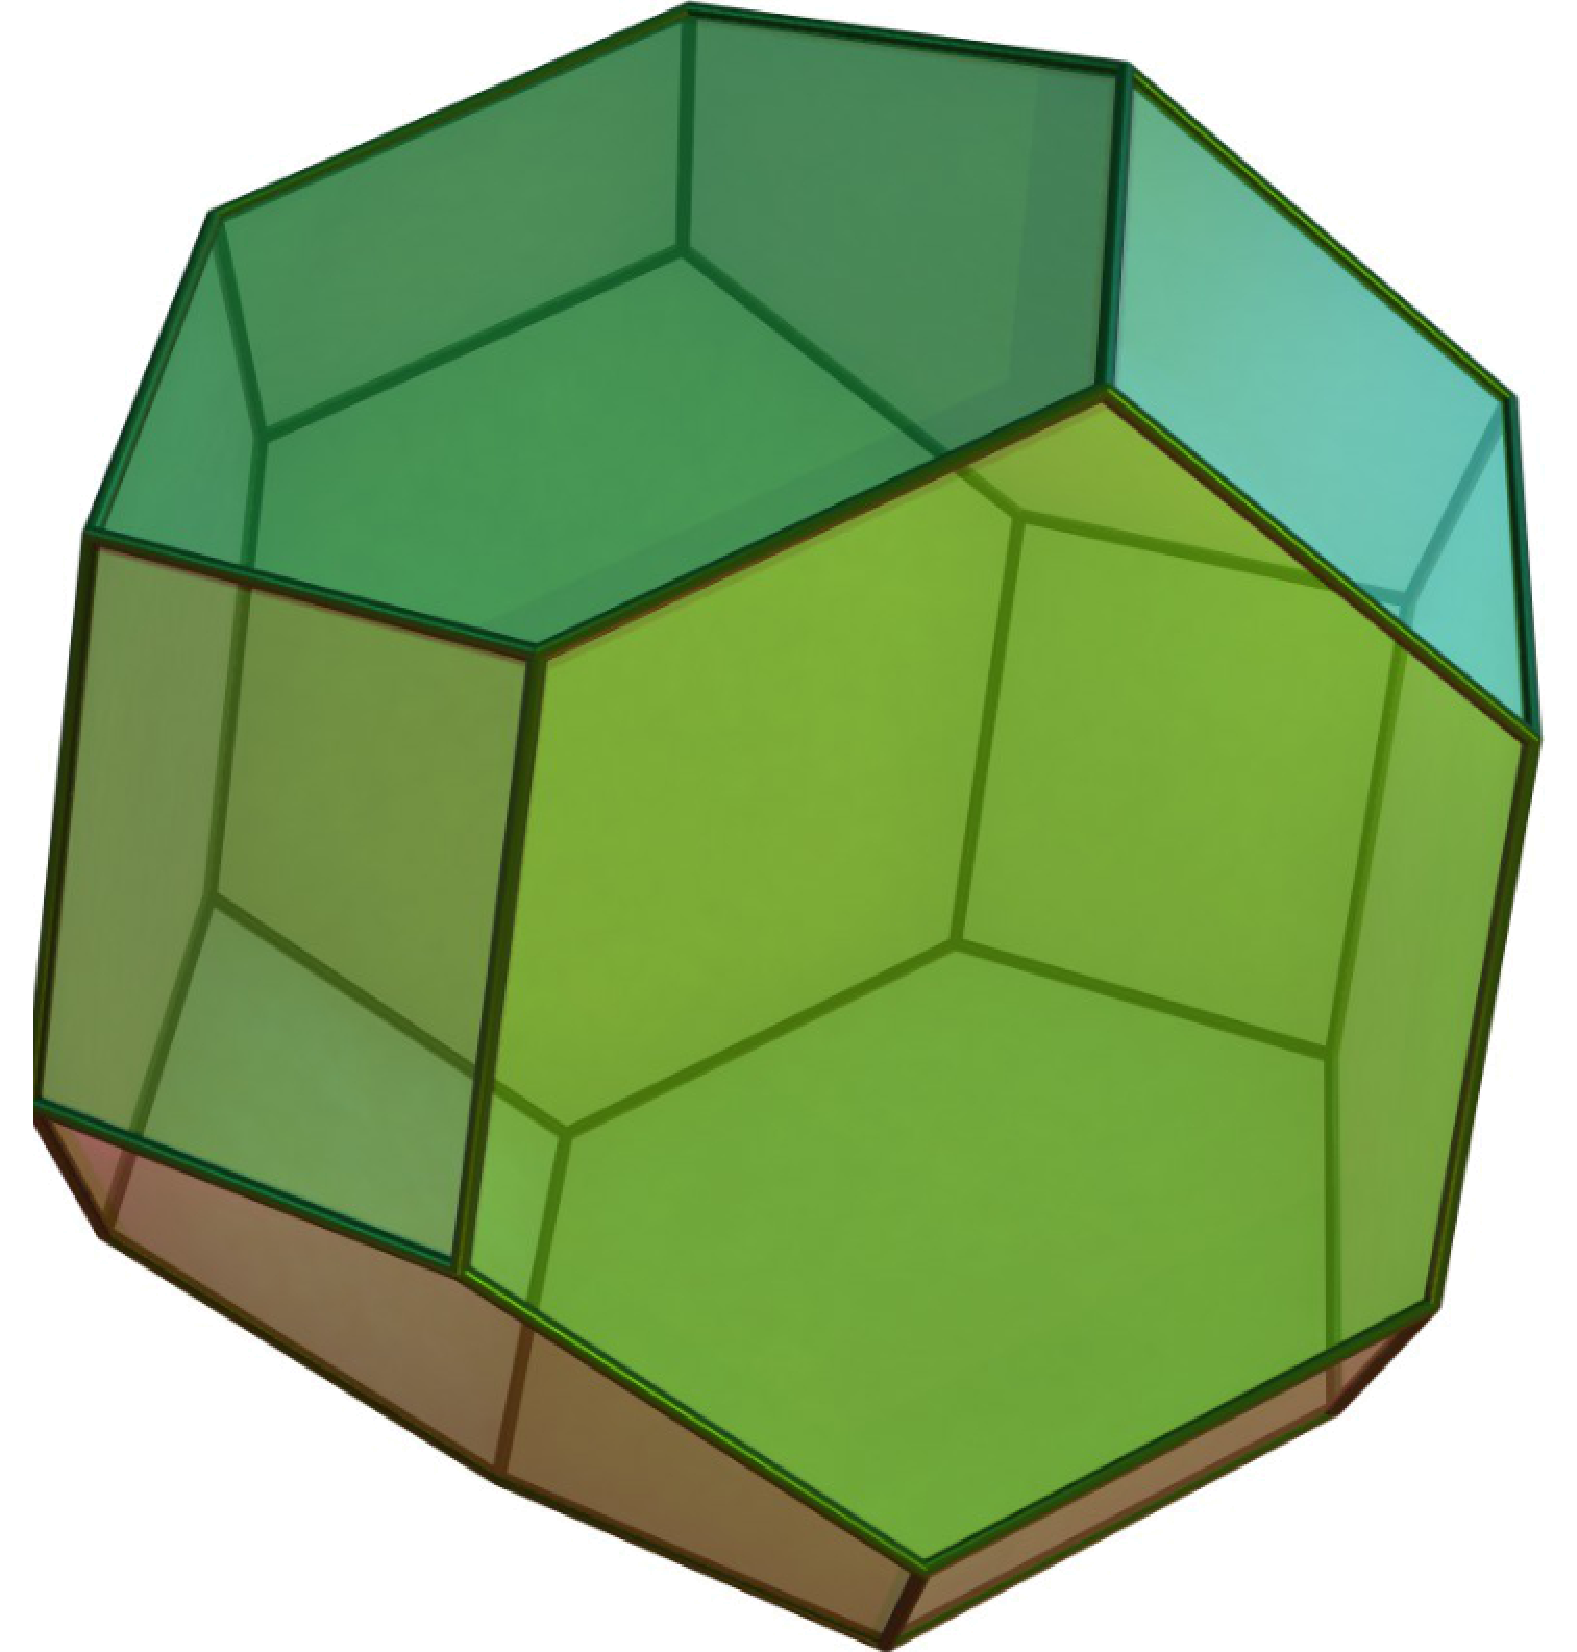
\includegraphics[width=7.25cm]{Truncatedoctahedron.pdf}
\end{figure}

	
	
	
	
	\section{Summary}
	
	An attempt is made to make more explicit the relationships of the various
	types of unit cell reduction used in crystallography.
	
	
	
	\ack{{\bf Acknowledgements}}
	
	Careful copy-editing by Frances C. Bernstein is gratefully acknowledged.
	
	Work by HJB funded in part by NIGMS (5P30GM133893-03 grant to BNL subaward to the Ronin Institute); 
	
	
	
	%-------------------------------------------------------------------------
	% The back matter of the paper - acknowledgements and references
	%-------------------------------------------------------------------------
	
	% Acknowledgements come after the appendices
	
	% References are at the end of the document, between \begin{references}
		% and \end{references} tags. Each reference is in a \reference entry.
	
	
	%-------------------------------------------------------------------------
	% TABLES AND FIGURES SHOULD BE INSERTED AFTER THE MAIN BODY OF THE TEXT
	%-------------------------------------------------------------------------
	
	% Simple tables should use the tabular environment according to this
	% model
	
	\bibliography{Reduced}
	
	\bibliographystyle{iucr}
	
	
	
\end{document}                    % DO NOT DELETE THIS LINE
%%%%%%%%%%%%%%%%%%%%%%%%%%%%%%%%%%%%%%%%%%%%%%%%%%%%%%%%%%%%%%%%%%%%%%%%%%%%%%
